\section{Widget Realizzati}
\label{chap:widget}
Per pensare e ideare una soluzione che permettesse di generalizzare la struttura dei widget e il loro trasferimento dati, durante il corso del progetto ne sono stati sviluppati diversi. All'interno della dashboard i widget sono stati suddivisi in due categorie: \textit{widget IT e widget Mobility}.
I primi mostrano dati relativi ai flussi interni gestionali della Loccioni, mentre i secondi riguardano dati che vengono generati dai test effettuati nelle \textit{stazioni di prova} dei macchinari.

\begin{figure}[ht]
\begin{center}
  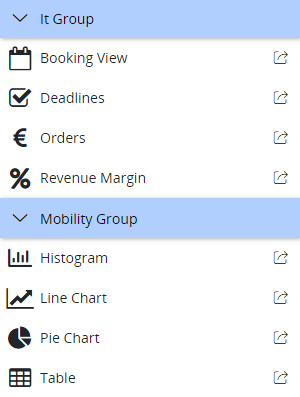
\includegraphics[width=4cm]{images/lista_widget.png}
  \caption{Lista dei widget realizzati}\label{fig:git}
\end{center}
\end{figure}
\FloatBarrier

\paragraph{Gruppo IT}
\begin{itemize}
    \item Booking view widget: 

\begin{figure}[ht]
\centering
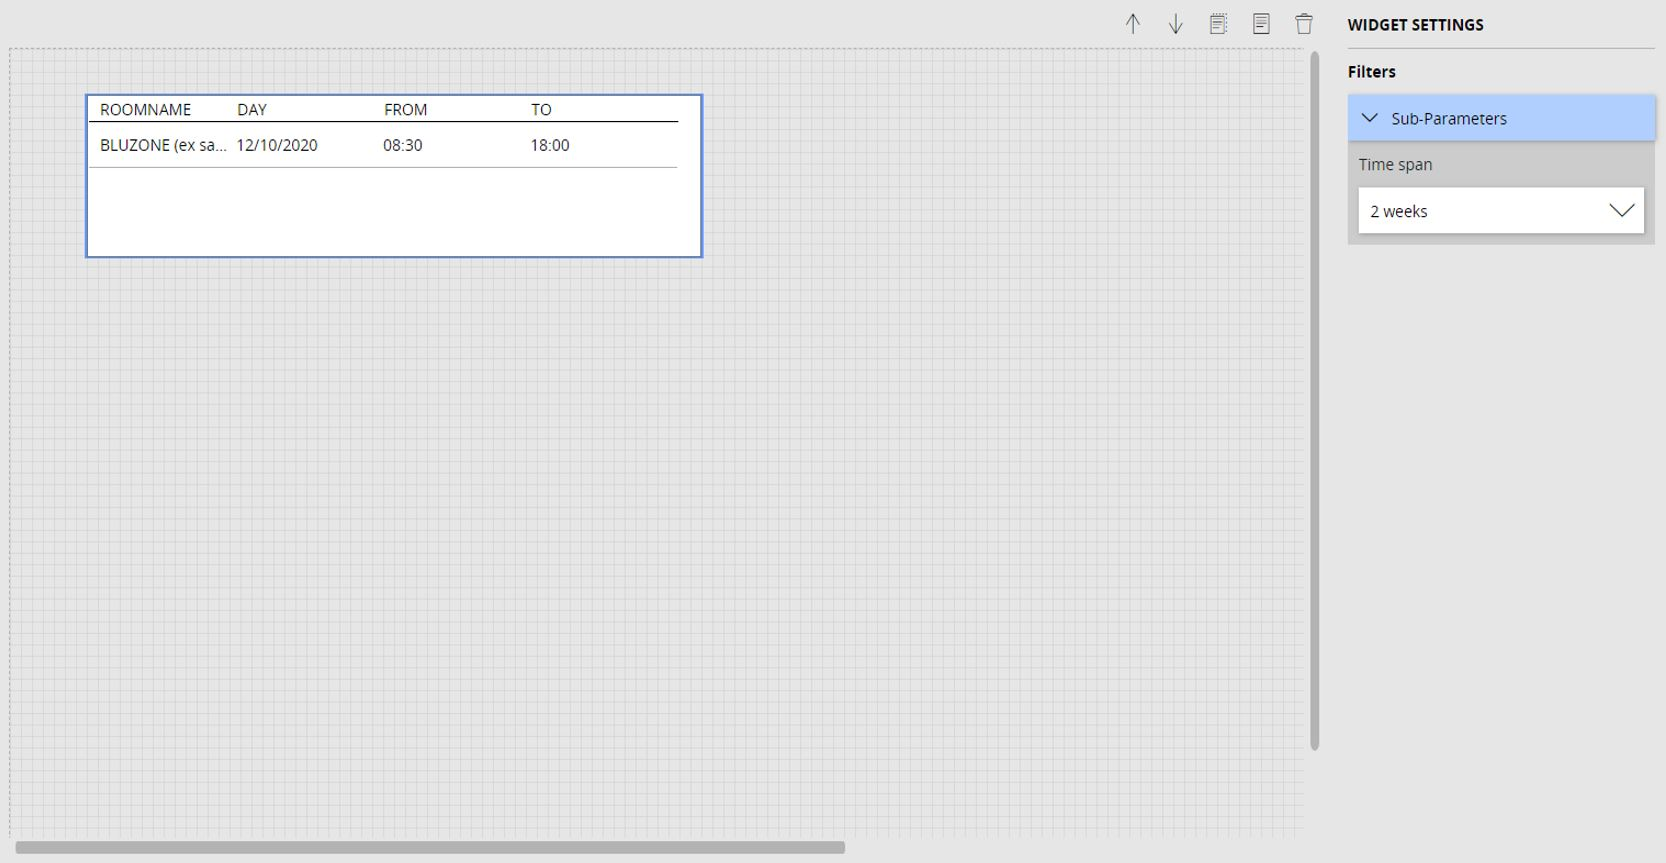
\includegraphics[scale=0.32]{images/BookingView.JPG}
\end{figure}
permette di visualizzare le prenotazioni dei salottini (stanze predisposte per effettuare riunioni). I parametri sulla destra filtrano i dati secondo l'arco di tempo selezionato, partendo dalla data corrente.
\end{itemize}
\pagebreak
\begin{itemize}
    \item Deadlines widget: 
    
\begin{figure}[ht]
\centering
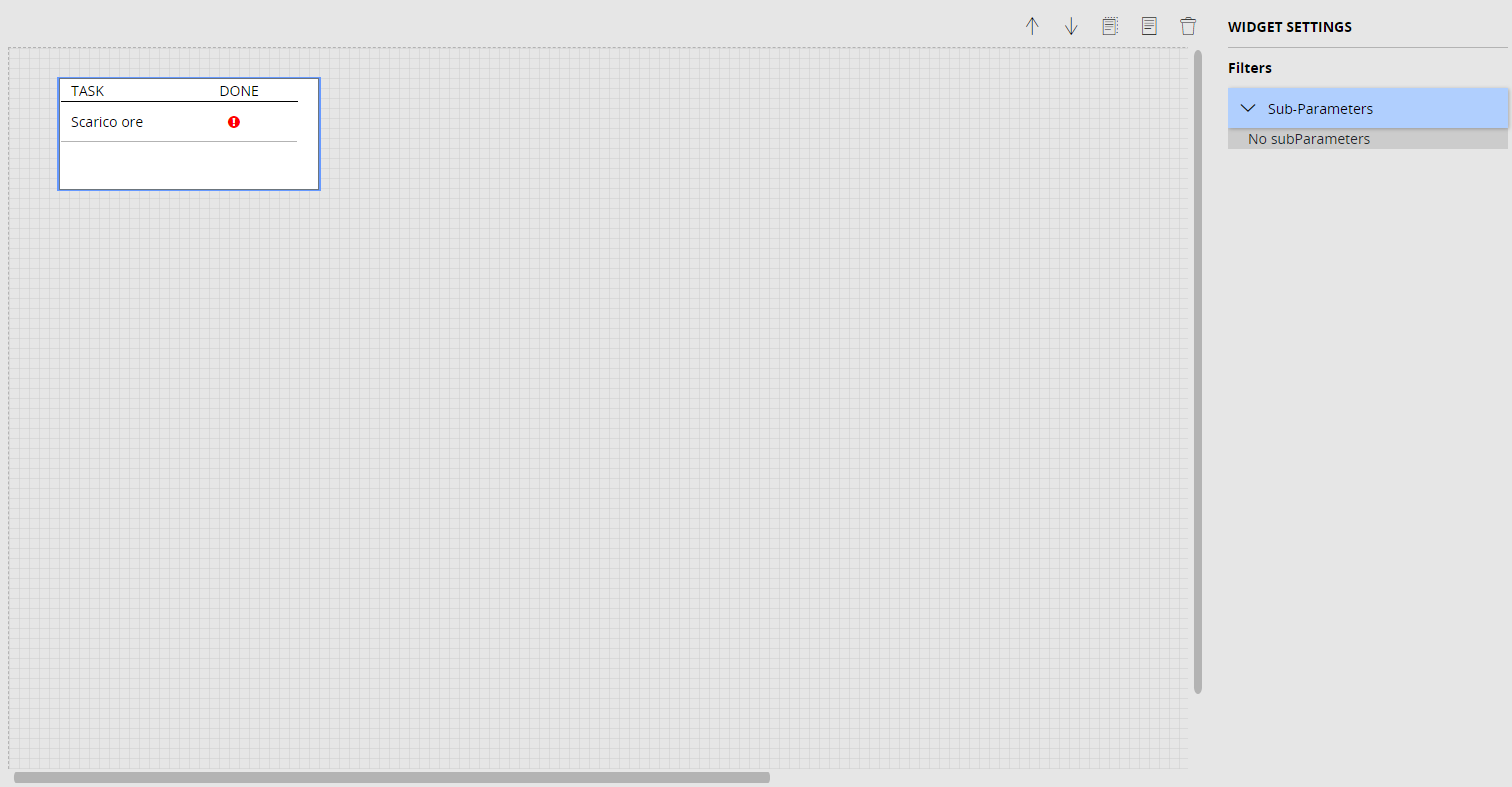
\includegraphics[scale=0.35]{images/Deadlines.png}
\end{figure}
permette di visualizzare un allarme in base alle scadenze dell'utente autenticato nel sistema.
\end{itemize}
\begin{itemize}
    \item Orders widget: 
    
\begin{figure}[ht]
\centering
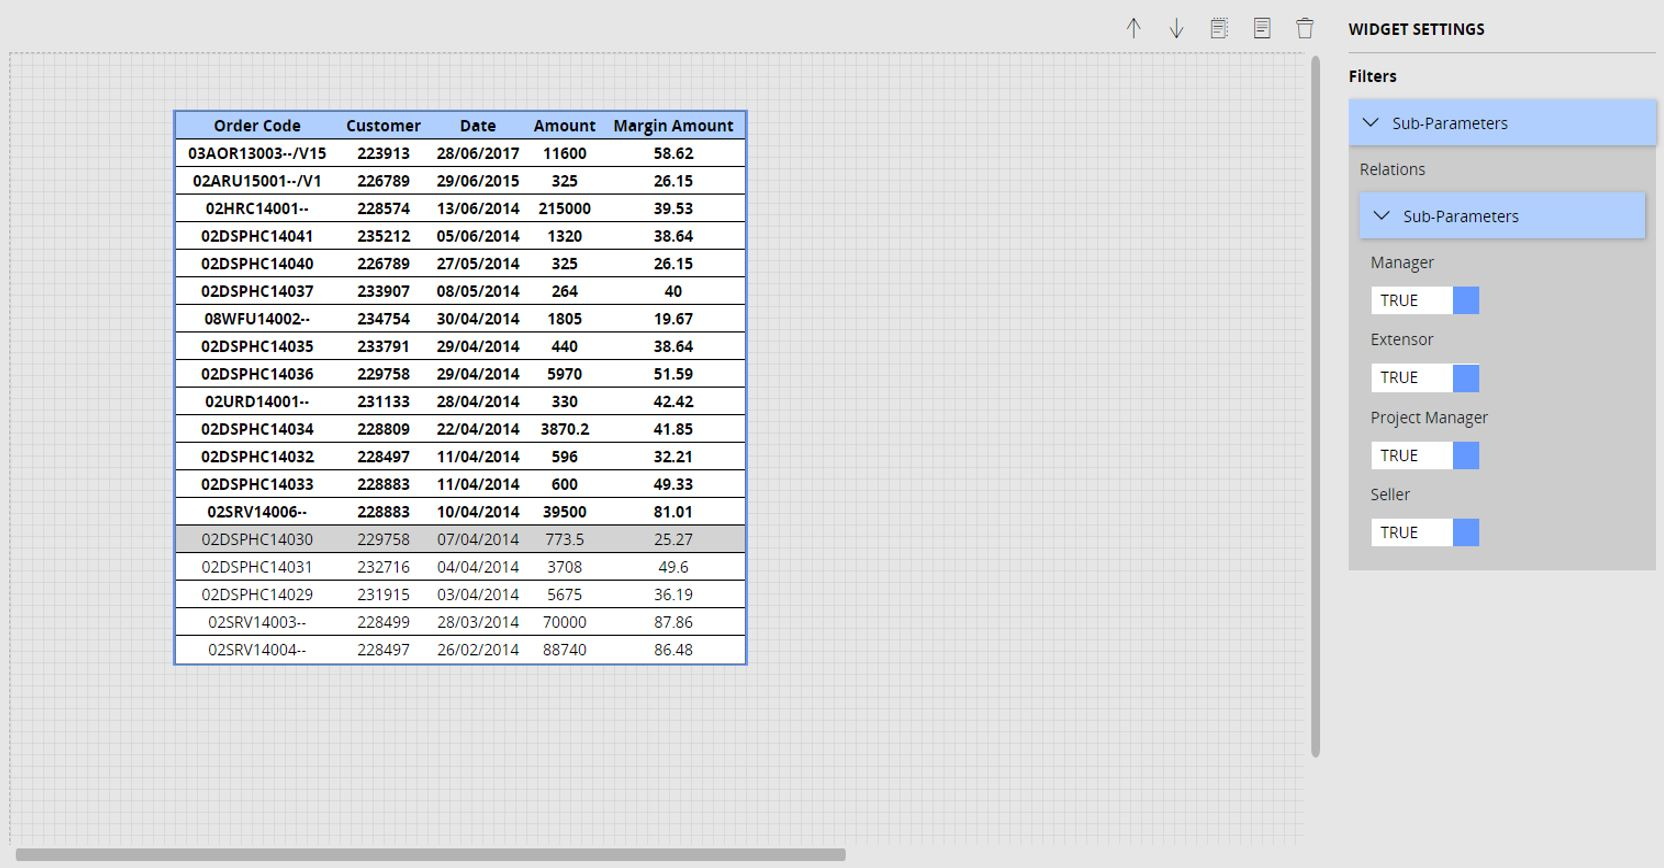
\includegraphics[scale=0.32]{images/Orders.JPG}
\end{figure}
permette di visualizzare informazioni relative agli ordini. I parametri sulla destra filtrano i dati in base al ruolo che l'utente ricopre per quell'ordine.
\end{itemize}
\pagebreak
\begin{itemize}
    \item Revenue margin widget: 
    
\begin{figure}[ht]
\centering
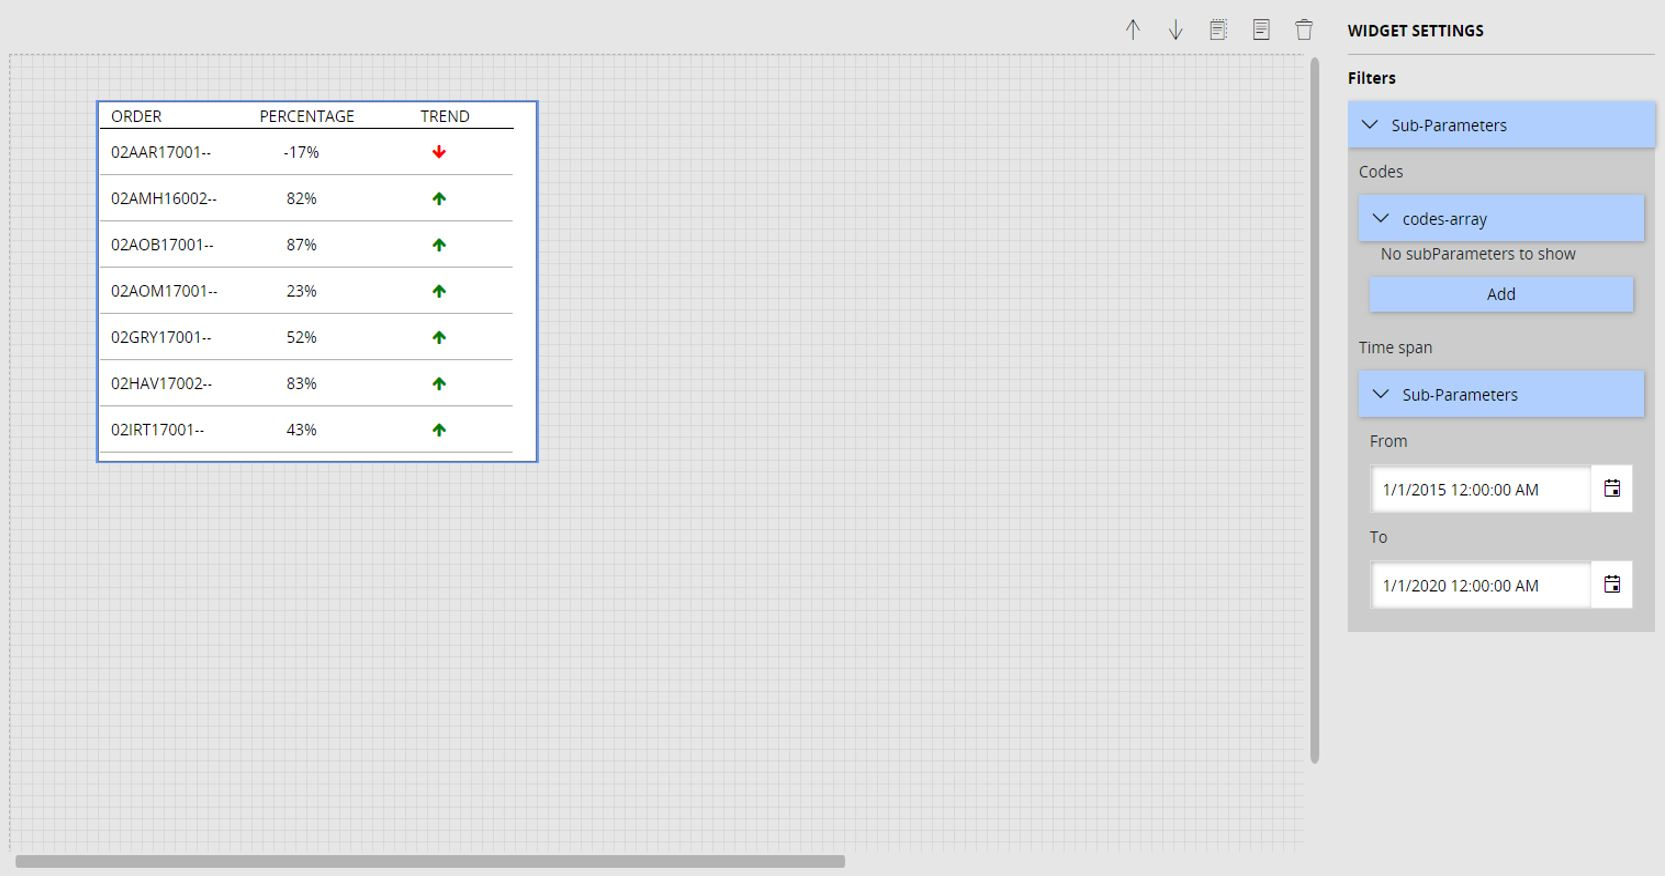
\includegraphics[scale=0.32]{images/RevenueMargin.JPG}
\end{figure}
permette di visualizzare il trend delle commesse e il valore in percentuale. I parametri sulla destra filtrano i dati in base all'arco di tempo selezionato e permettono di aggiungere ulteriori commesse al widget.
\end{itemize}
% FINE WIDGET IIIIIIIIIIIIIIIIIIT
\paragraph{Gruppo Mobility}
\begin{itemize}
    \item Histogram widget: 
    
\begin{figure}[ht]
\centering
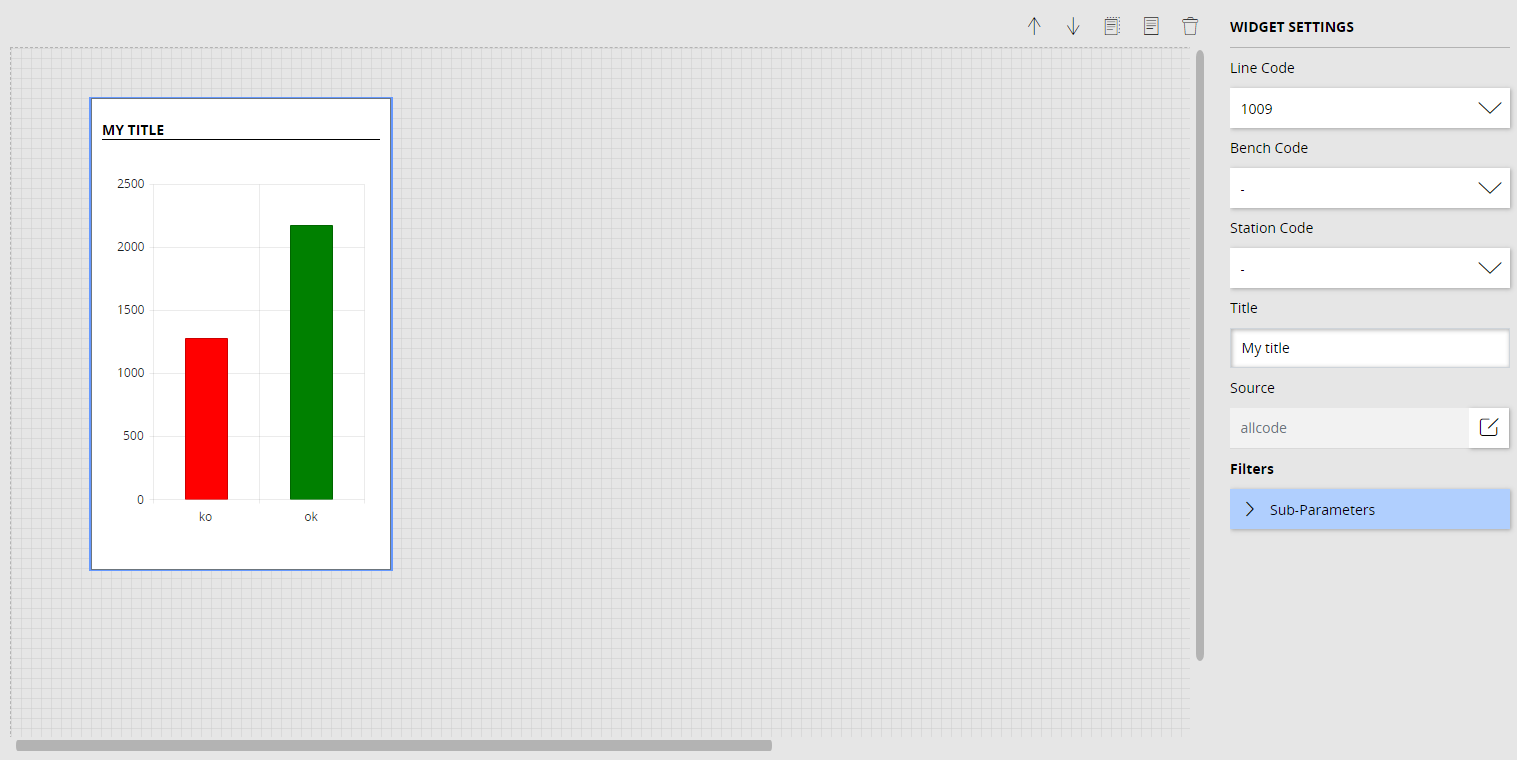
\includegraphics[scale=0.265]{images/Histogram.png}
\end{figure}
permette di visualizzare dati provenienti dalle macchine Loccioni in un grafico a istogramma. I parametri sulla destra filtrano i dati e permettono all'utente di selezionare la source da cui prendere i dati.
\end{itemize}
\pagebreak
\begin{itemize}
    \item Pie chart widget: 
    
\begin{figure}[ht]
\centering
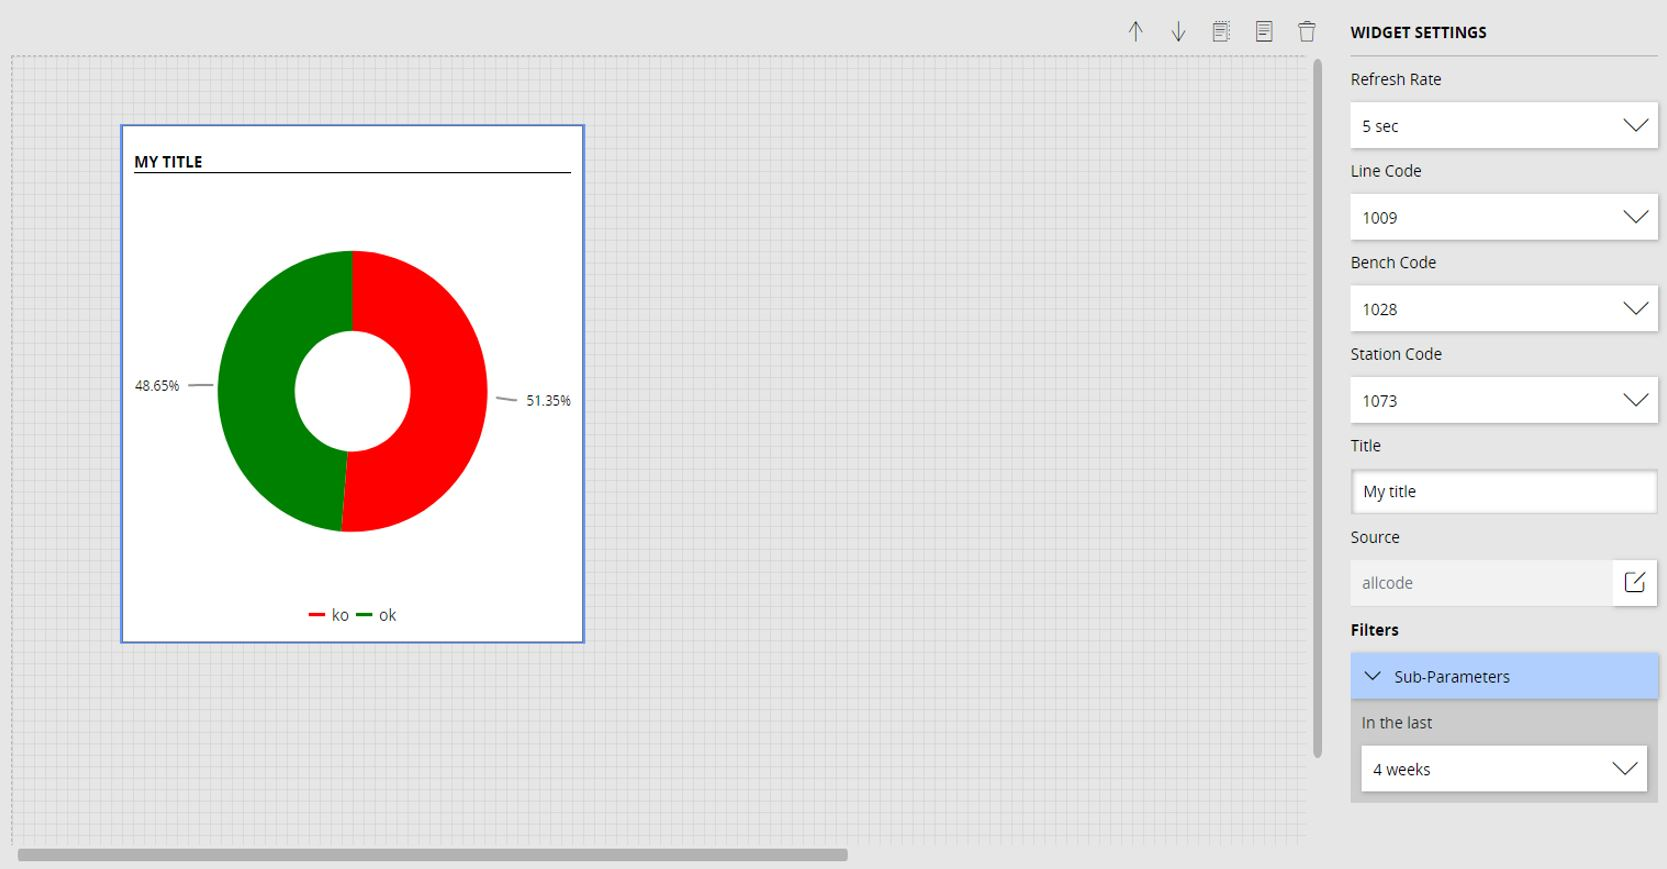
\includegraphics[scale=0.32]{images/Piechart.JPG}
\end{figure}
permette di visualizzare dati provenienti dalle macchine Loccioni in un grafico a torta. I parametri sulla destra filtrano i dati e permettono all'utente di selezionare la source e di cambiare l'intervallo di tempo in cui il widget ricarica i dati dal backend.
\end{itemize}
\begin{itemize}
    \item Line chart widget: 
    
\begin{figure}[ht]
\centering
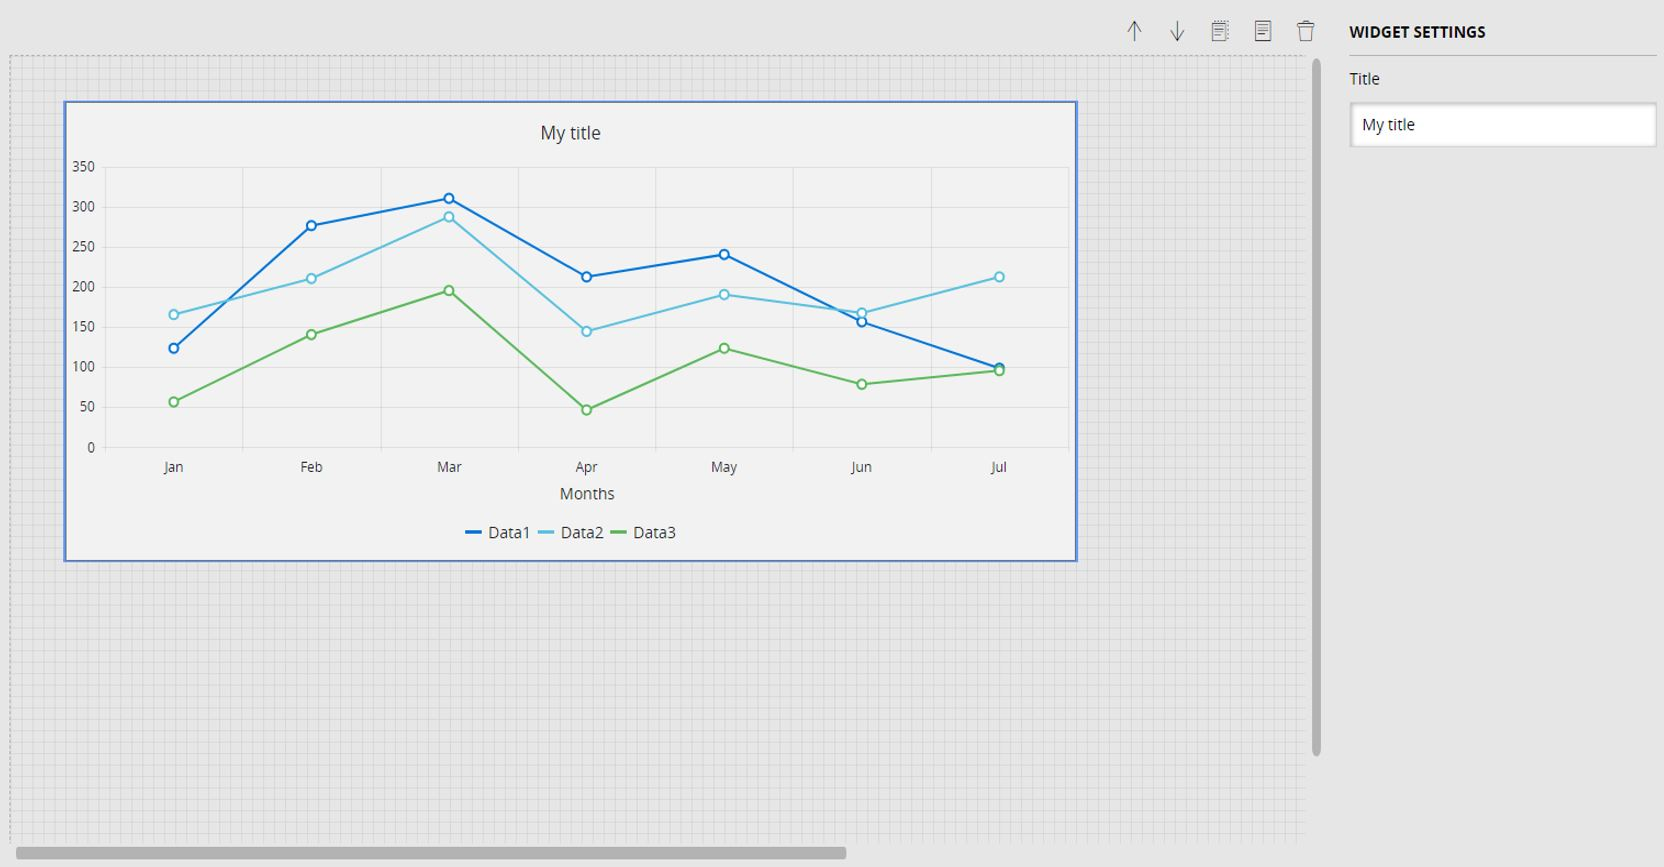
\includegraphics[scale=0.32]{images/Linechart.JPG}
\end{figure}
permette di visualizzare dati provenienti dalle macchine Loccioni in un grafico a linee.
\end{itemize}

\pagebreak
\begin{itemize}
    \item Table widget: 
    
\begin{figure}[ht]
\centering
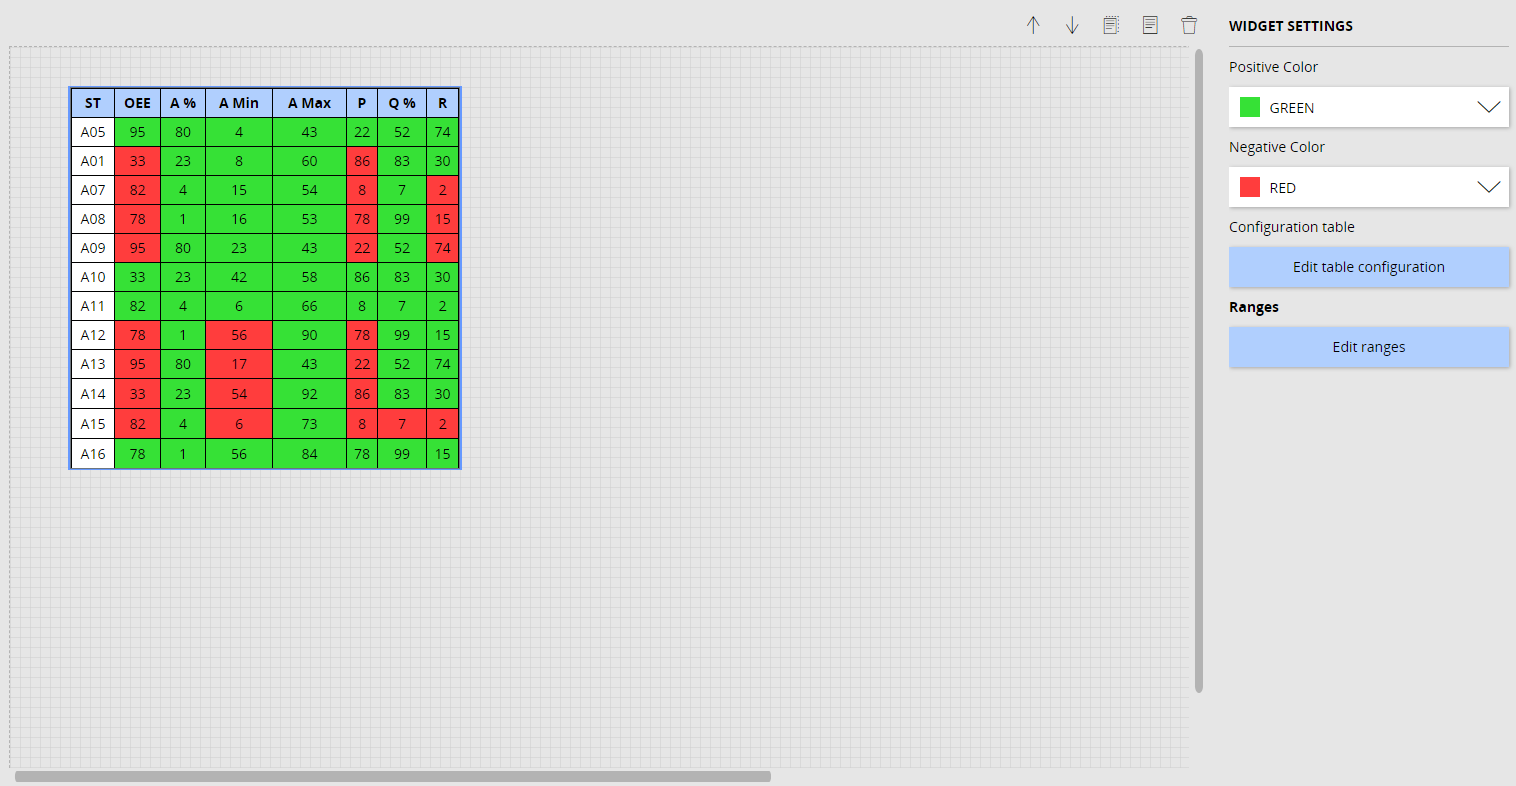
\includegraphics[scale=0.35]{images/Table.png}
\end{figure}
permette di visualizzare dati provenienti dalle macchine Loccioni in un grafico tabellare. I parametri sulla destra consentono all'utente di specificare le colonne e le righe che si vogliono caricare e consentono di impostare dei range secondo i quali un valore sarà visualizzato come positivo o negativo.
\end{itemize}
Il \textit{line chart widget} ed il \textit{table widget} non sono stati collegati ad alcun database e utilizzano quindi dati fittizi.